\documentclass[10pt]{beamer}
\usepackage{kotex}


% select theme  \usetheme{Hannover}Copenhagen
\usetheme{Copenhagen}
\usecolortheme{beaver}

\usepackage{kotex}
\usepackage{fancyvrb}
\usepackage{color}




\title{리버싱 스터디 발표}

\author{이윤승} 

\begin{document}

\begin{frame}
  \maketitle
\end{frame}


\begin{frame}{학습주제}
    \begin{itemize}
        \item 실행파일을 직접 까보자
    \end{itemize}

\end{frame}

\begin{frame}{Preface}
    \begin{itemize}
        \item 시작 인원 : 7 $\rightarrow$ 3
        \item 이윤승(스터디장) / 명현창 / 성호
        \item 이유는 모르겠지만 동아리 그만둔다고 나가는 사람이 매우 많았음.
    \end{itemize}
\end{frame}

\begin{frame}{스터디 진행}
    \begin{itemize}
        \item 딱 6번 만남. 9/29  11/24
        \item 디스코드 모임.
        \item 편차가 좀 있었지만 본인 기준 약 주당 5시간정도 소요
        \item 다음주 분량을 정하고 이에 대해서 각자 예습한후 (모르면 카톡방에서 질문) 모임날짜에 모여서 문제 푼것들 다시 복습.
        \item 예습하고 문제풀때는 화면공유하면서 다같이 진행
        \item 상대적으로 지식이 많은 스터디장이 최대한 관련지식을 알려주려고 노력
    \end{itemize}
\end{frame}


\begin{frame}{이동안 한것 (처음)}
    \begin{itemize}
        \item 드림핵의 reversing ver.1 강의로 시작
        \item 조원들이 어셈을 아는 사람들이 없었기에 일단 이 부분부터 강의보면서 공부함. 
        \item 처음엔 악으로 깡으로 x86 debug 파일 쓰면서 진짜로 어셈보면서 코드 읽어봤음.
    \end{itemize}
    \begin{figure}
        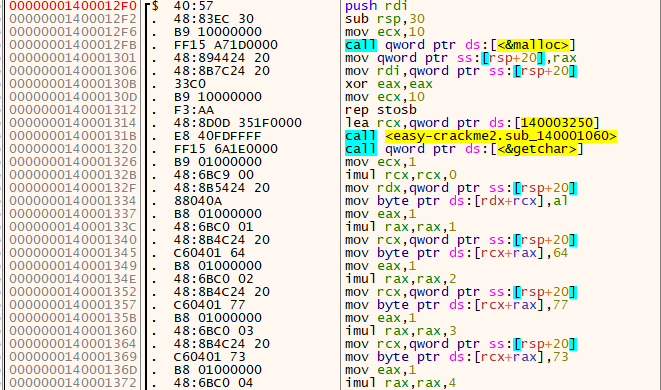
\includegraphics[width=0.6\columnwidth]{reversing.png}
    \end{figure}
\end{frame}

\begin{frame}{이동안 한것 (중간)}
    \begin{itemize}
        \item ver.1 다음에 reversing ver.2 가 있어서 다음은 이걸로 함.
        \item ida 도입으로 C 디컴파일 기능을 맛보고나서 신세계 체험중
        \item  C언어로 편하게 읽으면서 문제 난이도가 많이내려가서 꽤 어려운것도 할 수 있었음.
        \item 예제 문제로 실행파일을 직접 수정하는 문제도있었음.
        \item 몰랐는데 ver.1이 어려우니 쉬운걸로 나온게 ver.2더라
    \end{itemize}
    \begin{figure}
        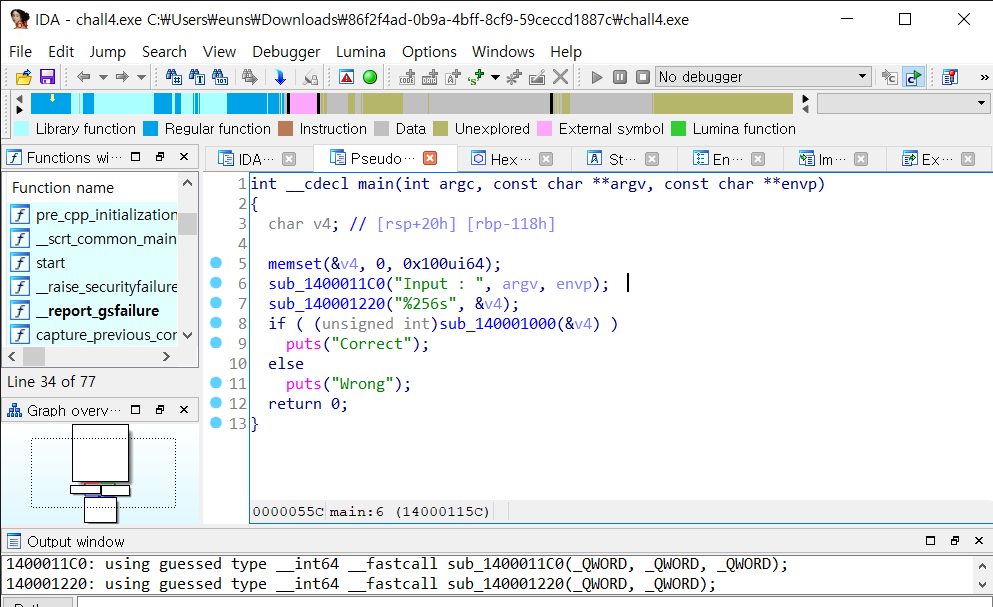
\includegraphics[width=0.6\columnwidth]{ida.png}
    \end{figure}
\end{frame}

\begin{frame}{이동안 (끝)}
    \begin{itemize}
        \item 실제 문제풀이
        \item CTF파트에 단계별 풀기 중 리버싱 문제를 순서대로 품.
        \item 여러 문제를 베타적으로 분배해서 각자 풀고 모여서 푼사람이 해설하면서 다른 사람이 다같이 푸는식으로 진행.
        \item 마지막 문제가 좀 많이 어려웠음.
    \end{itemize}
    \begin{figure}
        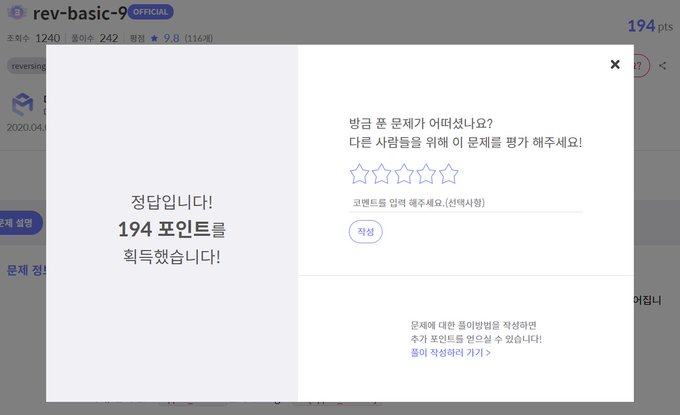
\includegraphics[width=0.6\columnwidth]{rev.jpg}
    \end{figure}
\end{frame}

\begin{frame}{결과}
    \begin{itemize}
        \item 총 11문제를 풀었음.
        \item 노력하면 어셈을 어느정도 읽을 수 있는 수준까진 도달
    \end{itemize}
\end{frame}


\begin{frame}{아쉬운점}
    \begin{itemize}
        \item 직접 푼 모든 문제가 프로그램에 들어가는 입력값을 뽑아내는 문제였음
        \item 다양한 유형의 문제를 풀지 (못)않은것 정도?
    \end{itemize}
\end{frame}

\end{document}